+\documentclass{udpreport}
\title{Metodos Numéricos : Tarea 1}
\author{Francisco Luna, Bastian Sepulveda, Fiorella Frigerio, Nicolas Ramirez }
\usepackage{amssymb}
\usepackage{amsmath}
\usepackage{graphicx}
\usepackage{float}
\usepackage{array}
\graphicspath{ {Imagenes/} }
\usepackage{listings}
\usepackage{color}




\begin{document}
\maketitle
\tableofcontents


\chapter{Introducción}

En el siguiente trabajo el principal objetivo fue analizar los tiempos de ejecución de los distintos métodos trabajados en Matlab. Para esto usaron varios métodos, como el de bisección, falsa posición, secante y Newton,  para encontrar las raíces de varias ecuaciones no lineales, y así poder comparar la efectividad de los métodos en cada ejercicio.

.
\chapter{Resolución de ecuaciones no lineales:}
\begin{enumerate}
\item Usando los métodos de bisección, falsa posición, y secante, encuentre la raíz aproximada 
de las siguientes ecuaciones no lineales en los intervalos indicados:

    \begin{enumerate}
        
    Para realizar estas ecuaciones se utilizaron los programas de :
    \begin{itemize}
        \item Biseccion.m
        \item Secante.m
        \item FalsaPosicion.m
    \end{itemize}
    y las comparaciones de error se hicieron en base a el resultado de la función fzero de matlab
    
    \item  \(x^3 - 4sen(x) +1 = 0\) , sobre [0,1] , [1,2].
        \begin{figure}[H]
            \centering
            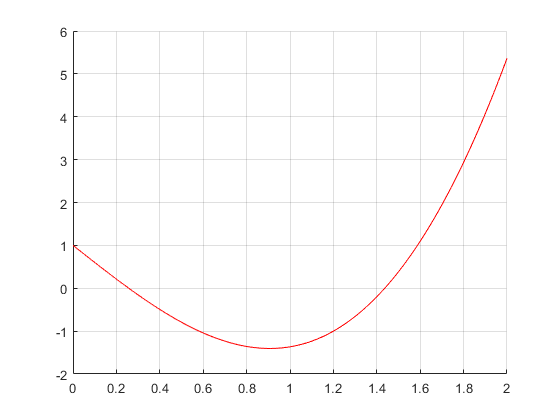
\includegraphics[width=9cm]{ec1.png}
             \caption{Gráfico Ej 1A}
        \end{figure}
        
            \begin{table}[H]Intervalo [0,1]:
            \centering
                \begin{tabular} { |c|c|c|c|}
                \hline
                Métodos       & Bisección & Falsa Posición & Secante  \\
                \hline
                Cero Obtenido &  0,2571       &    0,2571      &      0,2571    \\
                \hline
                Iteraciones   &    17        &     4     &       7        \\
                \hline
                Error Obtenido(\%) &       0      &       0      &     0         \\
                \hline
                Tiempo CPU &       0,009439     &      0,007311     &     0,002157         \\
                 \hline
                \end{tabular}
            \end{table}
            
        \begin{table}[H]Intervalo [1,2]:
        \centering
           \begin{tabular} { |c|c|c|c|}
                \hline
                Métodos       & Bisección & Falsa Posición & Secante  \\
                \hline
                Cero Obtenido &  1,4365       &    1,4364      &      1,4365   \\
                \hline
                Iteraciones   &    17        &    14     &       7        \\
                \hline
                Error Obtenido(\%) &       0      &       0,00696      &     0         \\
                \hline
                Tiempo CPU &       0,009656     &      0,016843    &     0,002164         \\
                 \hline
                \end{tabular}
            \end{table}
    
        
    \item \( e^{-t/2} +cos(2t) = 0 \), sobre [1,2].
    
        \begin{figure}[H]
            \centering
            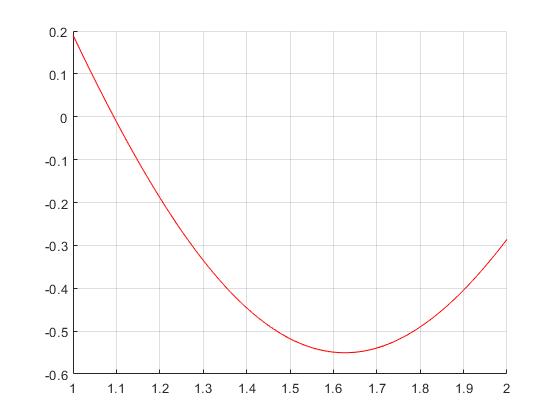
\includegraphics[width=8cm]{ec2.png}
            \caption{Gráfico Ej 1B}
        \end{figure}
        
        \begin{table}[H]
        \centering
           \begin{tabular} { |c|c|c|c|}
                \hline
                Métodos       & Bisección & Falsa Posición & Secante  \\
                \hline
                Cero Obtenido &  1.0940      &    1.0940     &      2,1852   \\
                \hline
                Iteraciones   &    17        &    14     &      7        \\
                \hline
                Error Obtenido(\%) &       0      &       0      &     99,74         \\
                \hline
                Tiempo CPU &       0,008504     &      0,006189    &     0,002032         \\
                 \hline
                \end{tabular}
            \end{table}
      
    \item \(x^3- e^{-x} +xsen(3x) = 0 \), sobre [0,2].\\
        
        \begin{figure}[H]
        \centering
        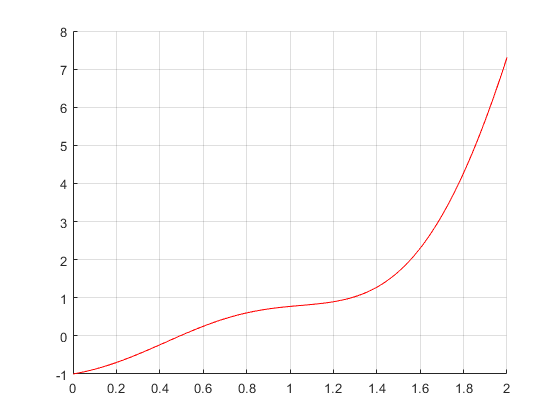
\includegraphics[width=10cm]{ec4.png}
        \caption{Gráfico Ej 1D}
        \end{figure}
        \begin{table}[H]
        \centering
           \begin{tabular} { |c|c|c|c|}
                \hline
                Métodos       & Bisección & Falsa Posición & Secante  \\
                \hline
                Cero Obtenido &  0,493      &    0,493     &      0,493   \\
                \hline
                Iteraciones   &   17        &    16     &      6     \\
                \hline
                Error Obtenido(\%) &       0      &       0      &     0         \\
                \hline
                Tiempo CPU &      0,008646     &      0,017988    &     0,001805         \\
                 \hline
                \end{tabular}
            \end{table}
        
    
    \item \(e^{-x^2} - cos(x) = 0 \), en [1,2].\\
        \begin{figure}[H]
            \centering
            \includegraphics[width=10cm]{ec3.png}
            \caption{Gráfico Ej 1C}
        \end{figure}
            \begin{table}[H]
            \centering
           \begin{tabular} { |c|c|c|c|}
                \hline
                Métodos       & Bisección & Falsa Posición & Secante  \\
                \hline
                Cero Obtenido &  1,448      &    1,448     &      1,448   \\
                \hline
                Iteraciones   &    17       &    10    &      6        \\
                \hline
                Error Obtenido(\%) &       0      &       0      &     0         \\
                \hline
                Tiempo CPU &       0,009362     &      0,007245    &     0,002157         \\
                 \hline
                \end{tabular}
            \end{table}
      

    
  
    Con una tolerancia de $10^{−5}$. Haga una comparación de los métodos en cuanto a la cantidad de iteraciones, el error cometido, tiempo de CPU. ¿Cual de ellos fue mas eficiente?.\\
    Si se comparan lo métodos por cantidad de iteraciones, el mas óptimo seria de la secante ya que al observar su curva se mantiene casi constantes y cubre menos área que las de los otros métodos, esto queda reflejado en el siguiente gráfico:
    \begin{figure}[H]
        \centering
        \includegraphics[width=10cm]{it.png}
        \caption{Gráfico cantidad de iteraciones.}
        \end{figure}
    Ahora si se compara por tiempos de ejecución, nuevamente el óptimo seria el método de la secante, lo cual queda demostrado en el siguiente gráfico:
    \begin{figure}[H]
        \centering
        \includegraphics[width=10cm]{tiempo1.png}
        \caption{Gráfico Tiempo CPU.}
        \end{figure}
    Continuando con las comparaciones, si en este caso se realiza por porcentaje de error, los métodos óptimos seria en primer lugar el de bisección ya que presento un error de 0\% en todas las funciones, luego vendría el de falsa posición que contada con un error casi despreciables, y finalmente el de la secantes, ya que en una función presento un error de casi el 100\%.
    Finalmente para concluir, el mejor método para utilizar, es el de la secante, aunque si la función tiene un comportamiento similar al de la ecuación b lo mejor seria optar por otro método.
      
    \newpage
    
    
    \end{enumerate}
\newpage
\item  Se desea calcular la raiz aproximada de las siguientes funciones utilizando el metodo de Illinois: 
    	\begin{enumerate}
    	\item  $f(x)= x^{10} - 1 =0$
    	\begin{figure}[H]
            \centering
            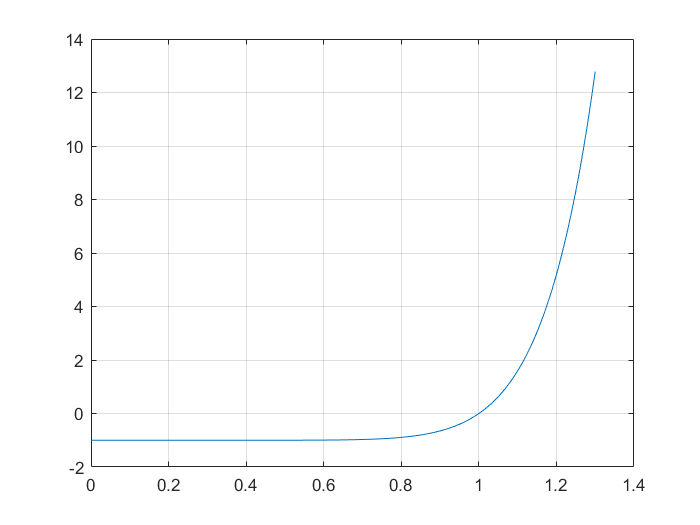
\includegraphics[width=7cm]{Ec21.png}
             \caption{Gráfico Ej 2a}
        \end{figure}
        \begin{table}[H]
            \centering
           \begin{tabular} { |c|c|c| }
                \hline
                Método       & Illinois & Falsa Posición  \\
                \hline
                Raíz Aprox. &  1      &    1       \\
                \hline
                Iteraciones   &    28       &    48          \\
                \hline
                \end{tabular}
            \end{table}
        
        \item $f(x)= cos(x) - x^3 =0$
        \begin{figure}[H]
            \centering
            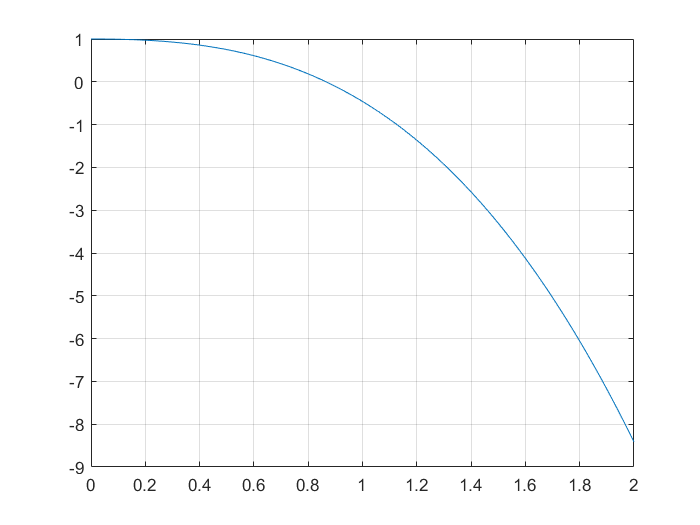
\includegraphics[width=7cm]{Ec22.png}
             \caption{Gráfico Ej 2b}
        \end{figure}
        \begin{table}[H]
            \centering
           \begin{tabular} { |c|c|c| }
                \hline
                Método       & Illinois & Falsa Posición  \\
                \hline
                Raíz Aprox. &  0.8655      &    0.8655       \\
                \hline
                Iteraciones   &    10       &    23          \\
                \hline
                \end{tabular}
            \end{table}
        
        \item $f(x)= sin(x) + sin(x^2) =0$
        \begin{figure}[H]
            \centering
            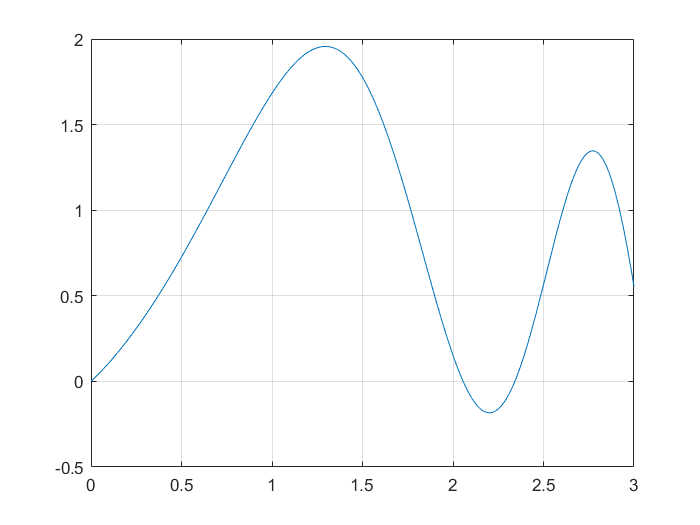
\includegraphics[width=7cm]{Ec23.png}
             \caption{Gráfico Ej 2c}
        \end{figure}
        \begin{table}[H]
            \centering
           \begin{tabular} { |c|c|c| }
                \hline
                Método       & Illinois & Falsa Posición  \\
                \hline
                Raíz Aprox. &  0      &    0       \\
                \hline
                Iteraciones   &    1       &    2          \\
                \hline
                \end{tabular}
            \end{table}
 Como se puede ver en las tablas, el método de Illinois converge más rápido que el método de falsa posición ya que el método de Illinois obtiene la raíz en menor cantidad de iteraciones. 
   
        
    \end{enumerate}
	

\item El dinero necesario para pagar la cuota correspondiente a un crédito hipotecario a interés fijo se suele
estimar mediante la denominada “ecuación de la anualidad ordinaria”:
\begin{center}
    $ Q = \frac{A}{i}(1-(1+i)^{-n}) $
\end{center}
donde Q es la cantidad pedida en préstamo, A es la cuota que debe pagar el beneficiario por el
préstamo, i es la tasa de interés fijado por la entidad bancaria que concede el préstamo y n es el
número de periodos durante los cuales se realizan pagos de la cuota.
Una pareja que desea comenzar una vida en común se plantea adquirir una vivienda y para ello saben
que necesitan pedir un préstamo de 50000 dólares a pagar trimestralmente durante un plazo de 25 años.
Sabiendo que para atender este pago pueden destinar una cantidad máxima de 800 dólares mensuales,
calcule cual es el tipo máximo de interés al que pueden negociar su préstamo con las entidades bancarias.¿Con dicho interés alguna de las entidades bancarias le concederá el préstamo solicitado?.
Hint.- Usar método de Newton, tomando como punto inicial i0 = 0.04.
Suponga ahora que desean endeudarse en 40 años en lugar de 25. Cual sería el interés en esta situación?


R:Mediante la ecuación de anualidad ordinaria, y remplazando  los datos obtenidos en el enunciado se obtuvo la siguiente ecuación
\begin{equation}
    50000=\frac{2400}{i}\left(1-\left(1+i\right)^{-75}\right)
\end{equation}
Donde nuestra función a iterar mediante el método de newton es (2.2), el cual usaremos como punto inicial i=0.03
\begin{equation}
    f(i)=\frac{2400}{i}\left(1-\left(1+i\right)^{-75}\right)-50000
\end{equation}
El resultado obtenido mediante el método de newton es de un interés igual al 13,8\%, el cual es un porcentaje viable para los bancos ya que se tendrá bastante ganancia de parte del banco. Para el caso de que quiera endeudarse en 16 años equivalentes a 32 periodos, su interés se ve aumentado en una cantidad igual al 14.8\%. Al ir aumentado los años de endeudamiento este converge a un valor de 15\%.\par



\item Considere la función \(f(x) = x*cos(x)-e^x+ 1\). % pregunta 5 
\begin{enumerate}
    
\vspace{0.9cm}
\item Considere las siguientes funciones. Realice unas 12 iteraciones de punto fijo, usando como puntos iniciales x0 = -0.5 y x0 = 0.5.\\ 


\begin{equation}
 g1(x) = \frac{e^x+x-1}
{1 + cos(x)}
\end{equation}
\\
\begin{itemize}
\item x0=0.5
\end{itemize}


\begin{table}[H]
    \centering
        \begin{tabular} { |c|c|}
        
        \hline
        iteración  &  Punto\\
        \hline
        1 &  0.6118        \\
         \hline
        2 &   0.8004       \\
         \hline
        3 &   1.1947       \\
         \hline
        4 &   2.5579      \\
         \hline
        5 &  87.3616      \\
         \hline
        6 & 4.7832e+37     \\
         \hline
        7 &  Inf         \\
         \hline
        8 &  NaN       \\
         \hline
        9 & NaN      \\
         \hline
        10 &   NaN       \\
         \hline
        11 &  NaN        \\
         \hline
        12 &   NaN        \\
        \hline
        
        \end{tabular}
    \end{table}
 
 \begin{itemize}
 \newpage
\item x0=-0.5
\end{itemize}
\begin{table}[H]
    \centering
        \begin{tabular} { |c|c|}
        
        \hline
        iteración  &  Punto\\
        \hline
        1 & -0.4759        \\
         \hline
        2 &  -0.4524        \\
         \hline
        3 &  -0.4298       \\
         \hline
        4 &   -0.4081      \\
         \hline
        5 &  -0.3875       \\
         \hline
        6 &   -0.3680     \\
         \hline
        7 &  -0.3497      \\
         \hline
        8 &  -0.3324       \\
         \hline
        9 &  -0.3163       \\
         \hline
        10 &  -0.3012       \\
         \hline
        11 &  -0.2871     \\
         \hline
        12 &  -0.2871       \\
        \hline
        \end{tabular}
\end{table}

\begin{equation}
 g2(x) = \frac{\sqrt{x(e^x-1)}}
{cos(x)}
\end{equation}
\\
\begin{itemize}
\item x0=0.5
\end{itemize}

\begin{table}[H]
    \centering
        \begin{tabular} { |c|c|}
        
        \hline
        iteración  &  Punto\\
        \hline
        1 &  0.6080       \\
         \hline
        2 &   0.7872     \\
         \hline
        3 &  1.1555       \\
         \hline
        4 &   2.4964     \\
         \hline
        5 & 0.0000 + 5.8994i        \\
         \hline
        6 &  0.1106 - 0.0106i       \\
         \hline
        7 & 0.1140 - 0.0113i         \\
         \hline
        8 &    0.1177 - 0.0121i     \\
         \hline
        9 &     0.1216 - 0.0130i     \\
         \hline
        10 &   0.1258 - 0.0140i       \\
         \hline
        11 &    0.1303 - 0.0151i   \\
         \hline
        12 &  0.1351 - 0.0163i        \\
        \hline
        
        \end{tabular}
        
    \end{table}
    \begin{itemize}
\item x0=-0.5
\end{itemize}

\begin{table}[H]
    \centering
        \begin{tabular} { |c|c|}
        
        \hline
        iteración  &  Punto\\
        \hline
        1 &  0.4735       \\
         \hline
        2 &   0.5676     \\
         \hline
        3 &  0.7171
       \\
         \hline
        4 &   0.9989     \\
         \hline
        5 & 1.7791        \\
         \hline
        6 &  0.0000 + 6.5089i      \\
         \hline
        7 &   0.0037 - 0.0660i       \\
         \hline
        8 &     0.0026 - 0.0660i   \\
         \hline
        9 &   0.0015 - 0.0660i       \\
         \hline
        10 &    0.0004 - 0.0660i      \\
         \hline
        11 &    0.0007 + 0.0659i \\
         \hline
        12 &   0.0004 - 0.0659i       \\
        \hline
        
        \end{tabular}
        
    \end{table}
 \vspace{3cm}   
 \item Teniendo en cuenta las siguientes funciones de iteración de punto fijo.  Realice unas 12 iteraciones de punto fijo, usando como puntos iniciales x0 = 0.5 y x0 = -0.5.\\   
  \begin{equation}
 g3(x) = x-2\frac{f(x)}
{f'(x)}
\end{equation}
 \begin{itemize}
\item x0=0.5
\end{itemize}

\begin{table}[H]
    \centering
        \begin{tabular} { |c|c|}
        
        \hline
        iteración  &  Punto\\
        \hline
        1 &      0.0846   \\
         \hline
        2 &    0.0041    \\
         \hline
        3 &   1.1230e-05 \\
         \hline
        4 &   8.4360e-11    \\
         \hline
        5 &    8.4360e-11  \\
         \hline
        6 &   8.4360e-11     \\
         \hline
        7 & 8.4360e-11    \\
         \hline
        8 &  8.4360e-11   \\
         \hline
        9 &   8.4360e-11      \\
         \hline
        10 &   8.4360e-11      \\
         \hline
        11 & 8.8.4360e-11  \\
         \hline
        12 &  8.4360e-11      \\
        \hline
        
        \end{tabular}
        
    \end{table}
     \begin{itemize}
\item x0=-0.5
\end{itemize}

\begin{table}[H]
    \centering
        \begin{tabular} { |c|c|}
        
        \hline
        iteración  &  Punto\\
        \hline
        1 &     2.3924  \\
         \hline
        2 &    0.6344   \\
         \hline
        3 &   0.1196 \\
         \hline
        4 &    0.0078   \\
         \hline
        5 &   3.9737e-05  \\
         \hline
        6 &   1.0509e-09    \\
         \hline
        7 & 1.0509e-09   \\
         \hline
        8 &  1.0509e-09  \\
         \hline
        9 &  1.0509e-09      \\
         \hline
        10 &  1.0509e-09      \\
         \hline
        11 & 1.0509e-09   \\
         \hline
        12 &  1.0509e-09     \\
        \hline
        
        \end{tabular}
        
    \end{table}
 \newpage
    
    \newpage
    \begin{equation}
 g4(x) = x-\frac{f(x)f'(x)}
{(f'(x))^2-f(x)f''(x)}
\end{equation}
\\
 \begin{itemize}

\item x0=0.5
\end{itemize}
\begin{table}[H]
    \centering
        \begin{tabular} { |c|c|}
        
        \hline
        iteración  &  Punto\\
        \hline
        1 &  -0.0551      \\
         \hline
        2 &    -0.0023   \\
         \hline
        3 &  -3.5887e-06 \\
         \hline
        4 &  1.2915e-10    \\
         \hline
        5 &    2.5829e-10  \\
         \hline
        6 &  2.5829e-10     \\
         \hline
        7 &     2.5829e-10 \\
         \hline
        8 &  2.5829e-10    \\
         \hline
        9 &       2.5829e-10   \\
         \hline
        10 &    2.5829e-10     \\
         \hline
        11 &    2.5829e-10 \\
         \hline
        12 &   2.5829e-10  \\
        \hline
        
        \end{tabular}
        
    \end{table}
     \begin{itemize}
\item x0=-0.5
\end{itemize}
\begin{table}[H]
    \centering
        \begin{tabular} { |c|c|}
        \hline
        iteración  &  Punto\\
        \hline
        1 &  -0.4614      \\
         \hline
        2 &   -0.3825   \\
         \hline
        3 &  -0.2366 \\
         \hline
        4 &  -0.0667    \\
         \hline
        5 &   -0.0035 \\
         \hline
        6 & -8.1704e-06     \\
         \hline
        7 &     -2.6233e-11 \\
         \hline
        8 &   -2.6233e-11   \\
         \hline
        9 &        -2.6233e-11 \\
         \hline
        10 &     -2.6233e-11    \\
         \hline
        11 &    -2.6233e-11 \\
         \hline
        12 &    -2.6233e-11  \\
        \hline
        \end{tabular}
    \end{table}
    
\item Que puede decir sobre el comportamiento de las iteraciones de punto fijo calculadas anteriormente.
\begin{itemize}

\item En la ecuación $g1$ en el momento de tomar de punto inicial 0.5 las iteraciones punto fijo divergen, mientras que si tomábamos como punto de inicio -0.5, las iteraciones divergían al punto -0.2871, lo que nos indica que este sea una posible solución de la ecuación.
\item En la ecuación $g2$ en ambos casos no divergieron a un valor en concreto las iteraciones, es mas incluso tenían parte imaginaria las iteraciones, lo que indica que esta ecuación no nos sirve para encontrar una posible solución.
\item En la ecuación $g3$ las iteraciones punto fijo para x0 = 0.5 convergian a 8,43 , y para x0= -0,5 esta convergia a 1.0509.
\item En la ecuación $g4$ en ambos casos converge a un valor especifico, el cual se aproxima harto a la solución, de los 4 casos mencionados anteriormente este es el que mas se aproxima a la solución, lo que indica que esta ecuación seria la mejor para determinar solución en este caso.
\end{itemize}


\end{enumerate}
\newpage

\item {\bf Métodos iterativos:} A continuación se describen algunos métodos de iteración de punto fijo que encuentran la raíz aproximada de f(x) = 0
\begin{itemize}
       
        
        \item Método de Schröder
            \begin{equation*}
                x_{n+1}=S_f(x_n)=x_n-\frac{f(x_n)f^{'}(x_n)}{f^{'}(x_n)^{2}-f(x_n)f^{''}(x_n)}
            \end{equation*}
        
        \item Método de aceleración convexa de Whittaker
            \begin{equation*}
                x_{n+1}=W_f(x_n)=x_n - \frac{f(x_n)}{2f^{'}(x_n)}(2 - L_f(x_n))
            \end{equation*}
        
\end{itemize}
	\begin{enumerate}
	
		\item Utilice los métodos para encontrar la solución de la ecuación no lineal $f(x)=0$, donde
		
		(i) $f_{1}(x)=xe^{x^2}-sen(x)+4cos(x)+6, en [-2,0].$
		
		\begin{table}[H]
			\centering
			\begin{tabular}{|c|c|c|c|}
				\hline
				Métodos & $x_{0}$ & Iteraciones & Cero Obtenido \\
				
				\hline
				Schroder & -2 & 2 & NaN \\
				\hline
				Whittaker & -2 & 10 & -1.3341 \\
				\hline				
			\end{tabular}
			\end{table}	
		
		
		
		(ii) $f_{2}(x)=x^3-3x^2(2^{-x})+3x(4^{-x})-8^{-x}, en [0,1].$
		
			\begin{table}[H]
			\centering
			\begin{tabular}{|c|c|c|c|}
				\hline
				Métodos & $x_{0}$ & Iteraciones & Cero Obtenido \\
				\hline
			
				Schroder & 0 & 4 & 0.6412\\
				\hline
				Whittaker & 0 & 68 & 0.6412\\
				\hline				
			\end{tabular}
			\end{table}	
			
		(iii) $f_{3}(x)=x^3 - e^{-x} + x*sin(3x), en [0,2].$	
		
		\begin{table}[H]
			\centering
			\begin{tabular}{|c|c|c|c|}
				\hline
				Métodos & $x_{0}$ & Iteraciones & Cero Obtenido \\
				\hline
			
				Schroder & -2 &  4 & -2.2895\\
				\hline
				Whittaker & -2 & 4 & -2.2895 \\
				\hline				
			\end{tabular}
		\end{table}		
\newpage			
		\item Compare los errores relativos vs. las iteraciones (mediante un gráfico) para los métodos (descritos
			anteriormente) que determinan la raíz de $f_{i}(x)=0$, para $i$ = 1,2,3.	
			\begin{itemize}
								
				\item Método de Schröder: 
				 \begin{figure}[H]
					\centering
					Por motivo que el valor converge a NaN no se puede realizar el gráfico de la función 1.
				\end{figure}
				
				\begin{figure}[H]
					\centering
					\includegraphics[width=10cm]{schroder2.jpg}
					\caption{Método de Schröder f2}
				\end{figure}
				\begin{figure}[H]
					\centering
					\includegraphics[width=10cm]{schoder3.jpg}
					\caption{Método de Schröder f3}
				\end{figure}
				 
				 
				 
				 \item Método de Whittaker;
				 \begin{figure}[H]
					\centering
						\includegraphics[width=10cm]{Whittaker1.jpg}
						\caption{Método de Whittaker f1}
				\end{figure}
				\begin{figure}[H]
					\centering
						\includegraphics[width=10cm]{Whittaker2.jpg}
						\caption{Método de Whittaker f2}
				\end{figure}
				\begin{figure}[H]
					\centering
						\includegraphics[width=10cm]{Whittaker3.jpg}
						\caption{Método de Whittaker f3}
				\end{figure}
			\end{itemize}
			
			
			
			Para resolver este problema, se ocuparon los archivos Newton5.m, schroder.m y whittaker.m.
        \end{enumerate}
\end{enumerate}
\newpage
\chapter{Resolución de sistemas de ecuaciones no lineales:}
    
        
        En los siguientes ejercicios, use como criterio de parada lo siguiente:
        \begin{center}
            $ \frac{|| x^{n+1} - x^{n} ||}{|| x^{n+1} ||} \leq 10^{-6} $  
        \end{center}
        

        Donde $||z||=\sqrt{z_{1}^{2} + z_{2}^2+...+z_{n}^{2}} , z \in \mathbb{R}^{n}$
    \begin{enumerate}   
        
        \item Considere los siguientes sistemas de ecuaciones no lineales\\
        
        \begin{math}
            (a)\left\lbrace
          \begin{array}{ll}
               x^3 - 3xy^2=1/2 \\\
                3x^2y-y^3 = sqrt(5)/2
            \end{array}
            \right.
            \hspace{3cm}
            (b) \left\lbrace
           \begin{array}{ll}
                 x^2+x-y^2&=1  \\
                 y-cos(x^2)&=0 
            \end{array}
            \right.
        \end{math}\\
        
        Usando el método de Newton, encuentre los puntos de intersección de las curvas descritas en los ítem (a) y (b). Para encontrar los puntos iniciales (x0,y0), apóyese en gráficos que le permitan encontrar una aproximación a la solución.
        
        
        Pregunta $ 1a) $\\
        
            
            $ Recta(1) : x^3 - 3xy^2=1/2 $
            
            $ Recta(2) : 3*x^2*y-y^3 = sqrt5/2 $
            
            \begin{figure}[h]
                \centering
                \includegraphics[width=15cm]{ec2sis.png}
                 \caption{Gráfico Ecuación Ej1A}
            \end{figure}
            
            
            Mediante las gráficas obtenida Figura 3.1, se puede visualizar que hay 2 intersecciones, una ubicada en el segundo cuadrante y la otra en el tercer cuadrante. Para encontrar la intersección de las curvas en el tercer cuadrante se utilizo el método de newton en varias variable con un punto inicial de $x0=[-3,-2]$, arrojando como resultado la intersección de las curvas generada en el punto $x=[-2.8401,-1.7708]$.\par Para calcular la intersección en el 2 cuadrante se procedió de la misma manera pero cambiando el punto inicial, el cual se utilizado  $x0=[-2,3]$, obteniendo como resultado la intersección en el punto $x=[-2.1401,1.4851]$.

        Pregunta $ 1b)$
        
            $ Recta(1) : x^2 + x -y^2=1 $
            
            $ Recta(2) : y-cos(x^2)=0  $
            \begin{figure}[h]
                \centering
                \includegraphics[width=15cm]{ec2sisb.png}
                 \caption{Gráfico Ecuación Ej1B}
            \end{figure}
            
         Observando la gráfica Figura 3.2 se aprecia que las curvan tienen 2 intersecciones,repitiendo el procedimiento ejecutado en el inciso a),para la intersección en el primer cuadrante se escoje el punto inicial $xo=[1.1] $ obteniendo como resultado $x=[0.8477,0.7526]$, para el calculo de la intersección en el tercer cuadrante utilizamos el punto inicial $x0=[-2,-1]$, obteniendo la intersección en $x=[-1.9143,-0.8662]$.
            
        Pregunta $ 2b) $\\
        
            
            $ Recta(1) (1-x)^2+100(y-x^2)$
                       
            \begin{figure}[h]
                \centering
                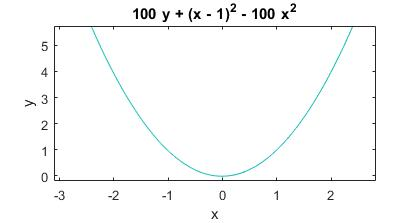
\includegraphics[width=15cm]{mnt2a.jpg}
                 \caption{Gráfico Ecuación Ej2A}
            \end{figure}
            
            
            Mediante las gráficas obtenida Figura 3.3, se puede visualizar que hay  intersecciones. Para encontrar la intersección de las curva se utilizo el método de newton en varias variable con un punto inicial de $x0=[-2,-3]$, arrojando como resultado la intersección de las curvas generada en el punto $x=[0.98401,2.0]$.\par el tiempo 3,29 segundos. En el caso del segundo punto no tiene solucion

        
           \end{enumerate}
    \newpage

    \chapter{Conclusión}
    
   Finalizando, podemos concluir que para el uso de ecuaciones no lineales  combinado con el uso de los métodos utilizados durante el informe, podemos ver en concreto el funcionamiento de cada método y respecto a esto cómo se comporta la función en cada método. Se pudo comprender que en casos como el método de Newton, secante, etc. La elección del punto fijo es clave para la eficacia del funcionamiento de los métodos, debido a que en caso de una elección errónea podría no haber convergencia local, debido a que la dependencia del punto dependerá la convergencia. 
   
   Finalmente la aplicación de los métodos estudiados son esenciales para la obtención de valores que comúnmente no podrían ser obtenidos de manera convencional, debido a la complejidad de estos. Este trabajo permitió comprender de manera práctica y fácil la teoría de los métodos numéricos estudiados.
      

\end{document}